\section{实验步骤}

\subsection{实验数据准备与检查}
标定数据位于\nolinkurl{work/asc/calibration}，包含六个静态姿态和六次转动；对准数据位于\nolinkurl{work/asc/alignment}。文件日期与GPS周内时刻对应2026年10月14日。表\ref{tab:data}中跨度是首末IMU时间戳之差。

\begin{table}[htbp]\centering\small
\caption{原始IMU数据规模}\label{tab:data}
\begin{tabular}{lrrl}\toprule
文件/用途&记录数&时间跨度/s&消息格式\\\midrule
\texttt{X\_up.ASC}&37570&187.845&RAWIMUSA\\
\texttt{X\_down.ASC}&46965&234.820&RAWIMUSA\\
\texttt{Y\_up.ASC}&38423&192.110&RAWIMUSA\\
\texttt{Y\_down.ASC}&36650&183.245&RAWIMUSA\\
\texttt{Z\_up.ASC}&37995&189.970&RAWIMUSA\\
\texttt{Z\_down.ASC}&38104&190.515&RAWIMUSA\\
\texttt{X\_down\_360.ASC}&37874&189.365&RAWIMUSA\\
\texttt{X\_down\_-360.ASC}&10889&54.440&RAWIMUSA\\
\texttt{Y\_down\_360.ASC}&10626&53.125&RAWIMUSA\\
\texttt{Y\_down\_-360.ASC}&9001&45.000&RAWIMUSA\\
\texttt{Z\_down\_360.ASC}&10152&50.755&RAWIMUSA\\
\texttt{Z\_down\_-360.ASC}&9640&48.195&RAWIMUSA\\
100C长静态对准&376820&1884.158374&RAWIMUXA\\\bottomrule
\end{tabular}\end{table}

逐条筛选IMU消息，检查字段数、时间单调性和CRC，共识别700709条有效IMU记录，未发现字段错误、CRC不匹配或重复/倒退时间。12个标定文件间隔均为0.005~s；对准文件有6处约0.010~s的间隔，最大为0.010001~s。

标定数据状态字均为零；
对准数据有9种状态字，
从\texttt{2d5f0000}至\texttt{2d670000}，
低16位均为零。

\subsection{六位置静态数据采集与截取}
\begin{figure}[htbp]\centering
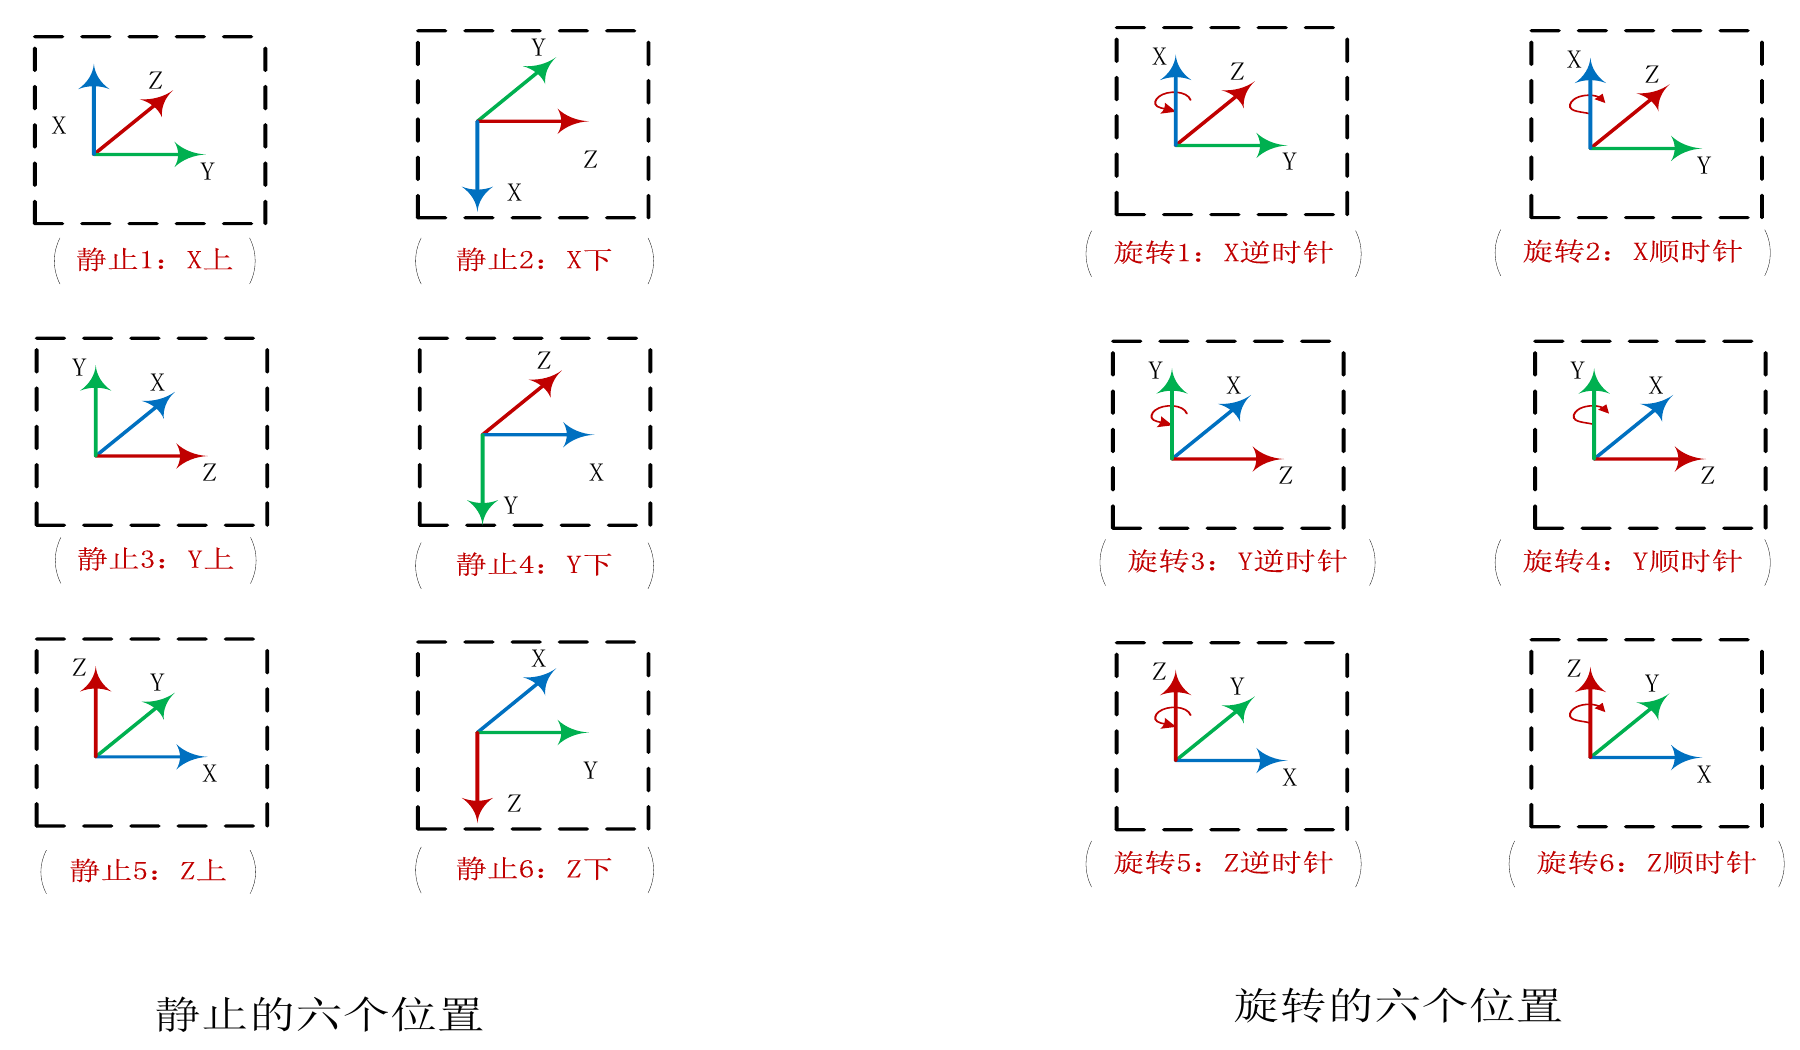
\includegraphics[width=1\textwidth]{guide_six_positions.png}
\caption{加速度计六位置与陀螺六位置旋转示意}\label{fig:sixpositions}
\end{figure}
图\ref{fig:sixpositions}左侧通过各轴朝上、朝下形成$\pm g$输入，右侧通过各轴正反转形成成对角位置输入。静态每位置5~min，陀螺以$10^\circ$/s转动$360^\circ$。转台依次使三个敏感轴铅垂朝上和朝下，每个姿态静置并采集；转动实验保持被测轴铅垂，正反各转一周。现有文件覆盖12类动作，六次主轴角速度平台约为$\pm10^\circ$/s。

六个静态文件统一剔除首尾各5~s后求均值，对各位置等权求解。选段样本数依次为35570、44965、36423、34650、35995、36104，有效增量时长为177.850、224.825、182.115、173.250、179.975、180.520~s。



\subsection{陀螺正反转数据截取}
\begin{figure}[htbp]\centering
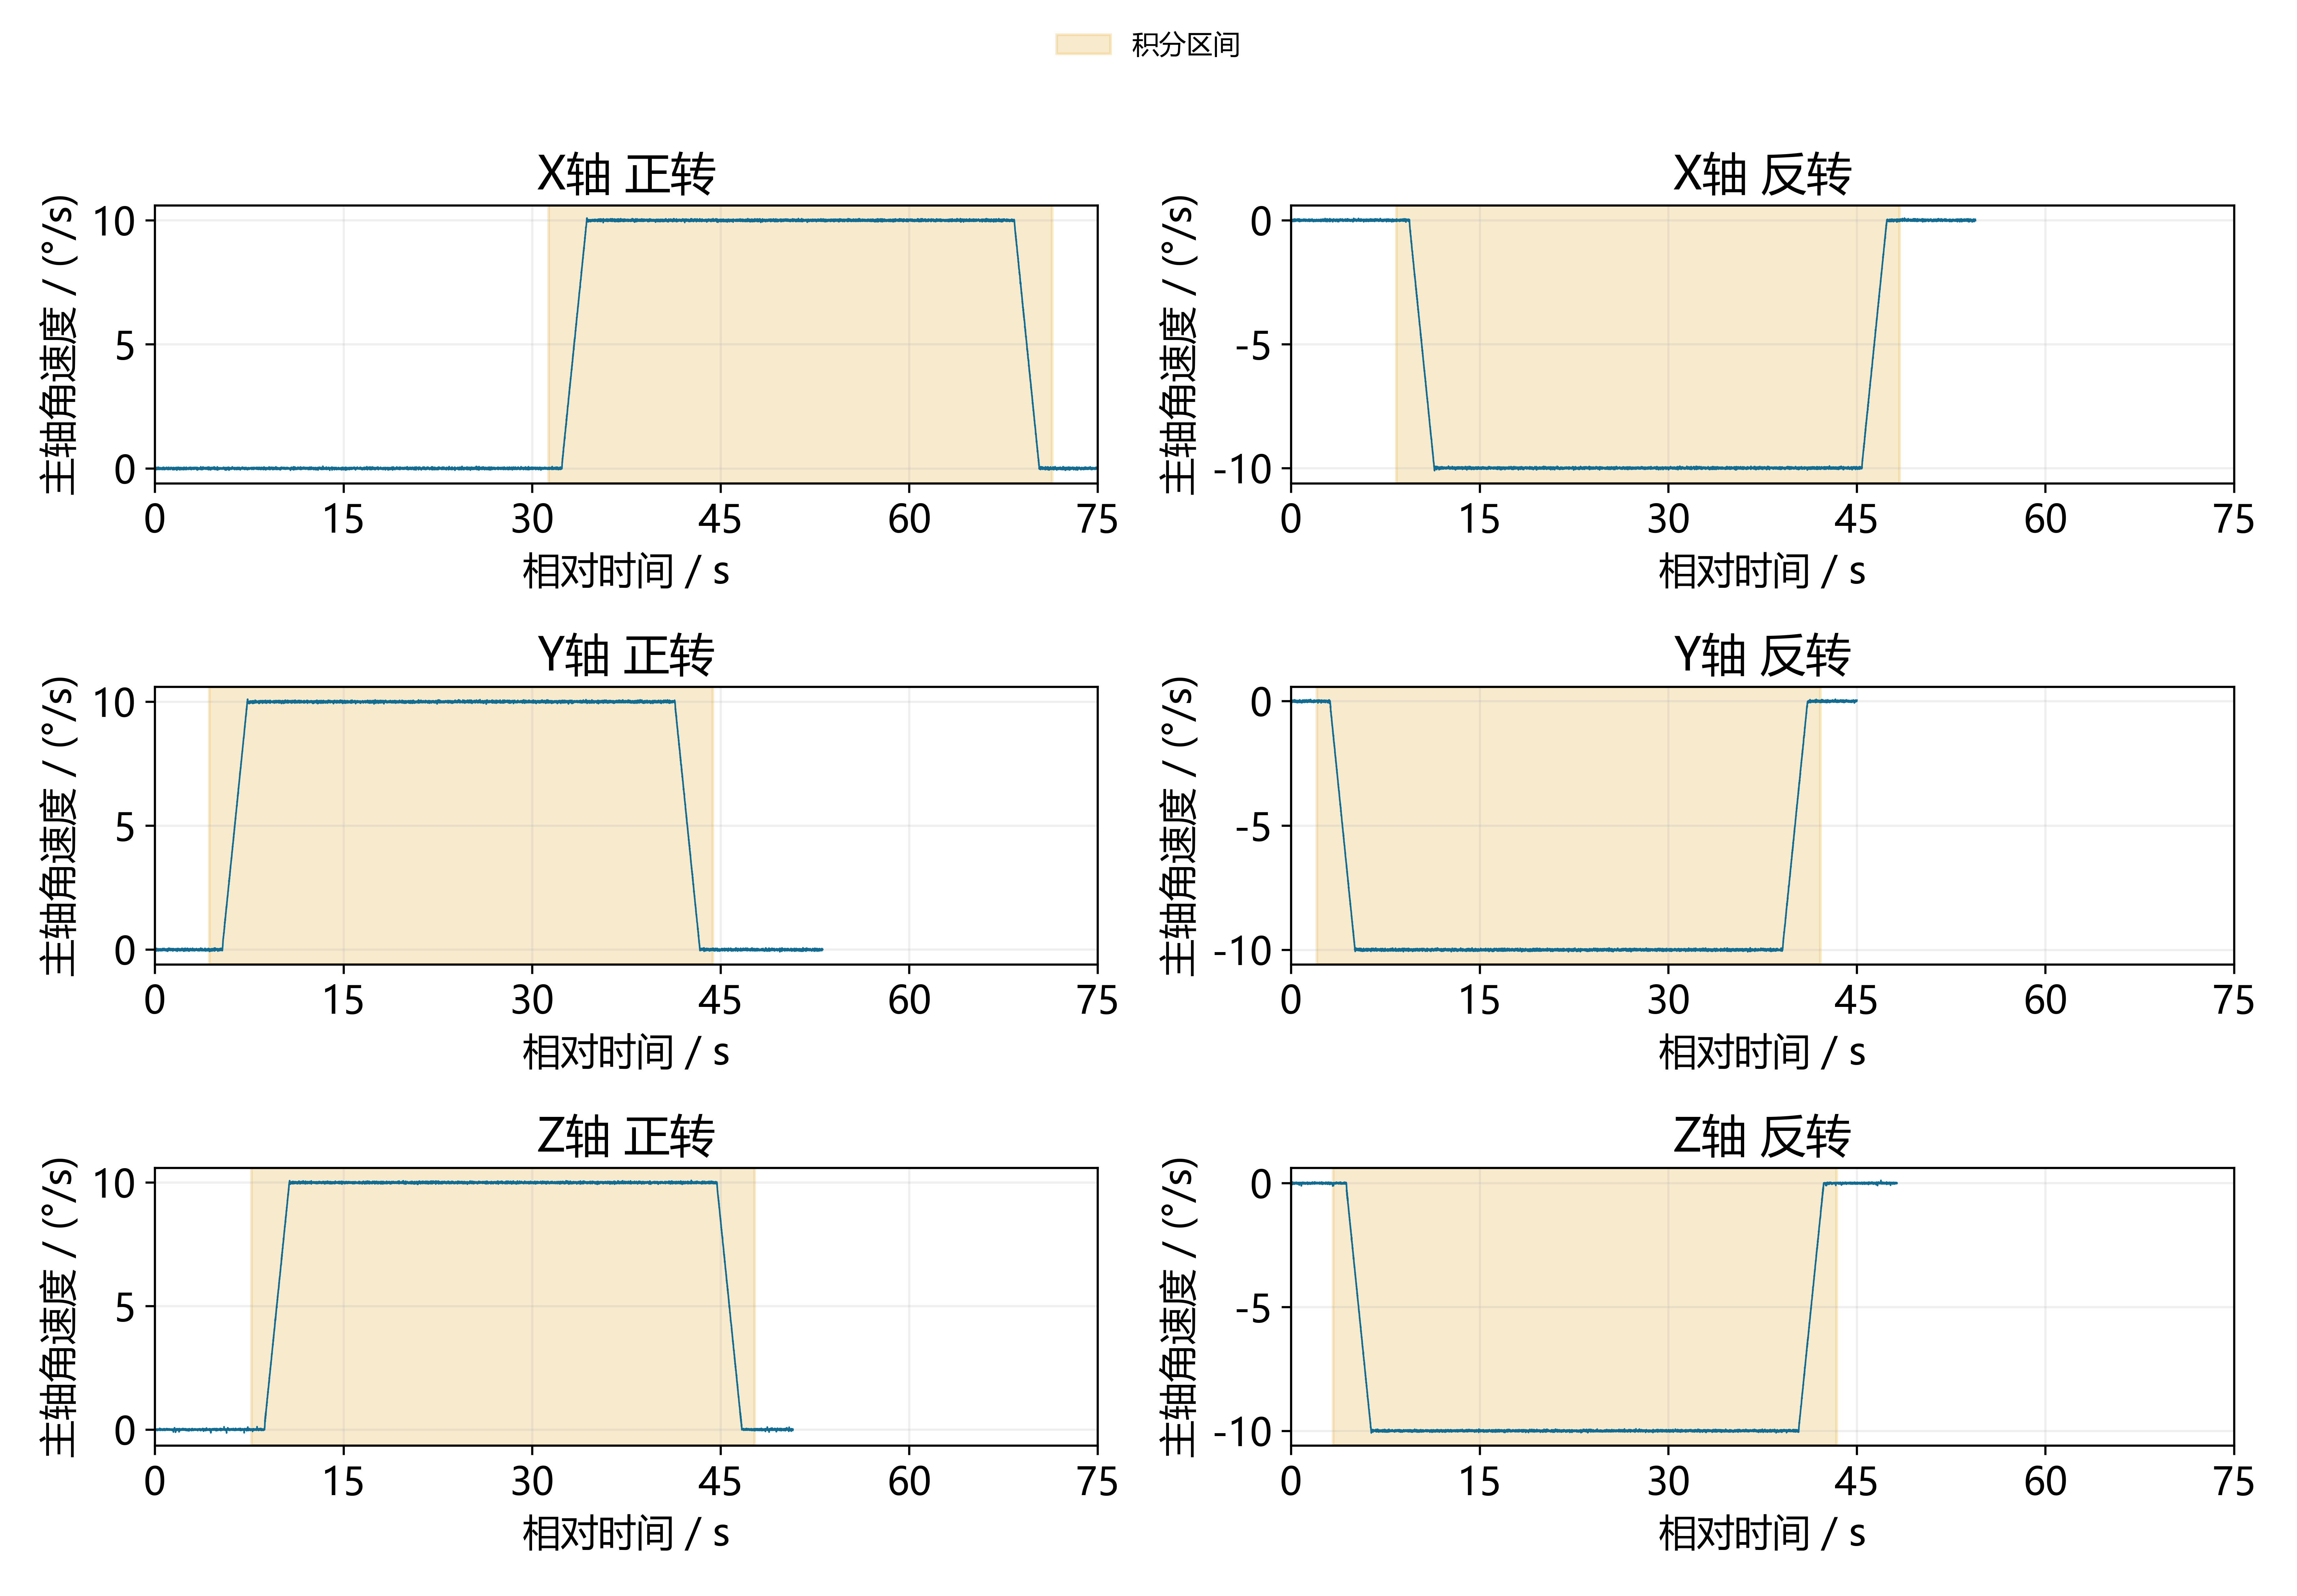
\includegraphics[width=0.85\textwidth]{gyro_rotation_windows.png}
\caption{六次主轴角速度与等长完整转动积分窗（阴影）}\label{fig:gyrowin}
\end{figure}
取文件首1~s主轴均值为基线，基线差做51点滑动平均，以$0.1^\circ$/s阈值识别活动范围。每对正反转取较长活动段长度，再增加400个样本作为前后约1~s静态留边，以相同样本数构造两个积分窗。图\ref{fig:gyrowin}显示各窗覆盖加速、匀速、减速和停稳；$X$正转原文件长189.365~s，不能与54.440~s的反转全文件直接配对。


\subsection{误差标定与补偿处理}
对六个静态位置分别计算三轴比力均值，由式\eqref{eq:accls}估计加速度计12个参数，并用式\eqref{eq:acccomp}补偿原始观测。对每轴正反转数据按等长完整区间累加角增量，计算比例因子；由对应朝上、朝下静态均值计算零偏。陀螺补偿先校正零偏和比例因子，比较转台角速度时再按敏感轴朝下扣除负的地球自转投影。内部角速度与零偏统一为rad/s，结果表将零偏换算为$^\circ$/h。

\subsection{静态解析粗对准处理}
整段解先平均376820条有效比力和角速度，再做一次双矢量定姿。每秒解以首条时间戳为起点，按$[t_0+j,t_0+j+1)$分组，平均该秒全部有效观测再解姿态；保留1884个完整秒窗，每窗199或200条，末尾不足一秒不计入每秒统计，逐历元解对每条独立定姿。
